\chapter{Contributions and a Computational Road Map}\label{chap:synthesis}

This book does not prove the Collatz conjecture. It does change what is known
about the problem, in three ways that are easy to lose among the details of
seventeen chapters: it adds a set of results, exact and quantitative, about the
map and about the optimizer the map suggests; it proves that a long list of
natural strategies cannot work, which narrows the space in which a proof can
live; and it corrects several claims, including some of our own. This chapter
collects all three in one place, with pointers to where each is proved and an
honest statement of what is new. It then uses them to lay out a computational
path to a solution: a staged programme in which every stage proves something
definite, the points where mathematics rather than computation must supply
the next step are marked, and the one route that could settle the whole
conjecture by finite computation is identified.

\section{The problem as the book leaves it}\label{sec:ch10d:state}

The conjecture is the conjunction of two statements that need different tools
(\cref{chap:path}).

The divergence half says that no orbit is unbounded. By the Ces\`aro identity\index{Cesaro identity@Ces\`aro identity}
(\cref{prop:cesaro}) it is equivalent to a law of large numbers along every
single orbit: the running mean $\bar k_N$ of the halving exponents
$\vt(3y_i+1)$ has lower limit strictly greater than $\lt\approx1.585$
(\cref{conj:cesaro}). The Bernoulli model predicts that the mean is $2$, and
Tao's theorem (\cref{thm:ch1:tao}) proves a version of this for almost every
starting value in logarithmic density, but nothing is known about any
particular orbit.

The cycle half says that the only cycle is $1\to2\to1$. By the periodic point formula
(\cref{cor:ch2:cycle} and the rational cycles of \cref{chap:cycles}) a cycle with $m$ odd steps among $k$ steps exists if and only
if some binary word $w$ of length $k$ with $m$ ones has $2^k-3^m$ dividing the
number $c_k(w)$ with a positive quotient. This is a divisibility question
about sums of terms $3^j2^i$, and it has nothing to do with averages.

The state of the art on each half, as of this writing, is the following.
Every starting value up to $2^{71}$ reaches $1$~\cite{barina2025}. Every
nontrivial cycle has at least $137\,528\,045\,312$ odd elements, by Hercher's
sharper accounting at that range; the exact certificate of \cref{thm:cycles} gives $72\,057\,431\,991$. No cycle has $m\le91$
ascending runs (Hercher, extending Simons and de Weger). At least $x^{0.84}$
integers up to $x$ reach $1$ (Krasikov and Lagarias), and by unrefereed preprints of 2026 by Mazur and by Lau, whose proofs the book does not check, a positive proportion do (\cref{chap:backward}). Almost every orbit attains
almost bounded values (Tao). The two halves are therefore both open, and in
both the obstruction is the same: every known method sees either an ensemble of
starting values or a bounded number of binary digits of one starting value, and the
conjecture is about every digit of every positive integer.

\section{What the book contributes}\label{sec:ch10d:contrib}

\Cref{tab:ch10d:contrib} lists the main results. The status column uses five
labels. \emph{New} means the result first appears in this book or in the
authors' earlier paper on Collatz dynamics. \emph{New proof} means the fact is
classical and the book gives a short, self contained proof in the form it needs.
\emph{Computed} means new exact numbers produced by the scripts of
\cref{app:code}. \emph{Corrected} means the book replaces an earlier claim,
ours or another's, by a correct one. \emph{Conditional} means the result assumes a statement the book does not prove, named in the cell. The Notes of each chapter give the
attributions in full; where a result builds on a named predecessor the table
says so.

\needspace{14\baselineskip}
{\small
\setlength{\tabcolsep}{3pt}
\begin{longtable}{@{}p{0.47\textwidth}>{\raggedright\arraybackslash}p{0.25\textwidth}>{\raggedright\arraybackslash}p{0.22\textwidth}@{}}
\caption{The main results of the book, with where they are proved and their
status.}\label{tab:ch10d:contrib}\\
\toprule
Result & Where & Status \\
\midrule
\endfirsthead
\toprule
Result & Where & Status \\
\midrule
\endhead
\bottomrule
\endfoot
\multicolumn{3}{@{}l}{\itshape Exact structure of the map}\\*
\addlinespace[2pt]
The halving exponent $\vt(3n+1)$ is exactly Geometric$(\half)$ on residue classes, and the Syracuse drift is exact & \cref{prop:geom}, \cref{cor:ch2:drift} & exact form of a classical heuristic \\
Martingale duality: $x_n$ a martingale, $\log x_n$ a strict supermartingale, the gap Jensen's & \cref{thm:martingale} & parts classical (Crandall; Lagarias and Weiss) \\
Parity autocorrelation $\rho(h)=(-\tfrac12)^h$ and the long run variance factor & \cref{thm:autocorr}, \cref{cor:longrun} & new \\
Exact stopping counts by a two term recursion & \cref{prop:ch2:dp} & Terras's recursion \\
Pathwise decomposition; the ten percent variance deficit of the stopping time sits at the bottom of the orbit (census to $2^{30}$) & \cref{prop:ch3:pathwise}, \cref{sec:ch3:missing} & computed; boundedness open (\cref{prob:ch11:o4}) \\
The third cumulant deficit behaves as an additive constant in the final descent; skewness predicted out of sample to $2^{49}$ & \cref{prop:ch16:deficit}, \cref{tab:ch16:o4} & computed; boundedness open (\cref{prob:ch11:o4}) \\
Uniform integrability fails, so optional stopping cannot be used & \cref{prop:uimartingale} & new proof \\
\addlinespace[4pt]
\multicolumn{3}{@{}l}{\itshape Cycles and continued fractions}\\*
\addlinespace[2pt]
Mediant lemma for the one sided distances $\lceil r\lt\rceil-r\lt$ & \cref{lem:ch8:mediant} & new proof (Hercher's Lemma 22) \\
Every nontrivial cycle has $r\ge72\,057\,431\,991$ odd elements, with an exact integer certificate of $44$ rungs & \cref{thm:cycles}, \cref{sec:ch8:certificate} & method Eliahou's, bound Hercher and Puchert's; certificate new \\
Verification thresholds: where extending the verified range moves the bound & \cref{tab:ch8:thresholds} & computed \\
Diophantine insufficiency: no irrationality measure plus verification excludes all cycles & \cref{prop:ch8:insufficient} & new form of a point of Halbeisen and Hungerb\"uhler; corrects our paper \\
Window lemma: an arithmetic margin of order $m/3$ would exclude all cycles & \cref{lem:ch8:window}, \cref{cor:ch8:window} & new \\
Machine checked statements in Lean & \cref{sec:ch8:lean} & new \\
Erd\H{o}s $125$ density exact to $4^{17}$; depth of minima a function of the fractional part of $m\log_43$ & \cref{sec:ch16:p7} & computed \\
\addlinespace[4pt]
\multicolumn{3}{@{}l}{\itshape Divergence, counting and residues}\\*
\addlinespace[2pt]
Ces\`aro identity: divergence is equivalent to a running mean at most $\lt$ & \cref{prop:cesaro} & new formulation \\
Model chain modulo $3^a$ exactly stationary after $a$ strides; the apparent spectral gap modulo $27$ is spurious & \cref{lem:ch9:mixing}, \cref{rem:ch9:oddreps} & restates an identity of Tao; computed \\
Certified exponents for the inverse tree, $x^{0.477}$ integers reach $1$ & \cref{thm:ch5b:exponent}, \cref{cor:ch5b:count} & new proof of a weaker classical bound \\
Residue certificates of every depth fail on a closed null set containing $-1$, $-5$, $-17$ & \cref{prop:ch10b:residue} & new statement \\
Residue sieve grows like $2^{0.95k}$, the exponent $H(1/\lt)$ & \cref{sec:ch10b:divergence} & computed \\
Bregman decomposition of orbits; uniform dissipation $c_*=D(7/9)$ per Syracuse step & \cref{prop:ch7b:bregman}, \cref{prop:ch7b:dissipation} & new \\
Given the positive density theorems and the verification to $2^{71}$, logarithmic density one of the orbits reaching $1$, and so a bounded form of Tao's theorem, implies the conjecture & \cref{prop:ch9b:bounded} & new; conditional on the unrefereed preprints of Mazur and Lau \\
Step counts of the positive density theorems below $3\cdot10^6$; the exact $3$ adic offset law to level $18$; the backward tree from $1$ below $2^{24}$ & \cref{sec:ch9b:steps}, \cref{sec:ch9b:offsets}, \cref{tab:ch9b:tree} & computed \\
\addlinespace[4pt]
\multicolumn{3}{@{}l}{\itshape Majorization pressed to its limit}\\*
\addlinespace[2pt]
The cycle inequality is the descent inequality of the multiplicative majorizer & \cref{prop:ch5c:cyclemm} & reformulation of the classical cycle identity \\
No potential $\log x+\varphi(x\bmod2^k)$ certifies descent, for any $k$ & \cref{thm:ch5c:residue} & new \\
Surplus along chains; the block map and its descent frequency & \cref{prop:ch5c:surplus}, \cref{prop:ch5c:block} & surplus new; block map from Terras and Steiner \\
Run length potentials $\log x+c\,\vt(x+1)$ fail, in the model, on more than $14.3$ percent of odd integers for every $c>\log(3/2)$ & \cref{prop:ch5c:runpot} & new \\
\addlinespace[4pt]
\multicolumn{3}{@{}l}{\itshape Simulation}\\*
\addlinespace[2pt]
Two horizons: level sets of $\tau$ are clopen, those of $\sigma_\infty$ have no $2$ adic description & \cref{prop:ch10b:horizons} & new \\
Perfect split sampling of the exceptional classes at any depth, $O(k)$ per draw & \cref{thm:ch10b:perfect} & new \\
Coalescence or independence for local moves in deep level sets & \cref{prop:ch10b:acceptance} & new \\
Slow integers below $2^B$ form a small number of trees of merged orbits & \cref{tab:ch10b:clusters}, \cref{tab:ch10b:trees} & computed \\
\addlinespace[4pt]
\multicolumn{3}{@{}l}{\itshape The optimizer}\\*
\addlinespace[2pt]
Two steps of Switching MM are gradient steps of sizes $\alpha$ and $(1+\beta)\alpha$ on quadratics & \cref{thm:smmquad} & new \\
Exact stationary variance; noise amplification below $5/3$ for every $\beta<1$ and every step & \cref{thm:smmvar}, \cref{prop:ch7:uniform} & new; corrects the halving heuristic \\
Gain weight theorem: no periodic schedule beats gradient descent's noise floor at matched speed & \cref{thm:ch7:gainweight}, \cref{cor:ch7:nobeat} & new \\
Exact joint spectral radius; every switching rule is stable if the transient bound conjecture holds & \cref{prop:ch5b:jsr}, \cref{cor:ch5b:anyswitch} & new; the second part conditional on \cref{conj:ch5b:transient} \\
Linear rate on smooth strongly convex functions, exact in the worst case & \cref{thm:ch5b:rate} & new \\
Rate and noise frontier for period two steps; multiplicative noise thresholds & \cref{prop:ch7:pareto}, \cref{prop:ch7:mult} & new \\
Convex rate of Switching MM by three point inequalities, a factor $1+\beta/2$ better than gradient descent when $1+\beta\le\varphi$ & \cref{thm:ch7b:smmrate} & new \\
Exact convex worst case of Switching MM: two branch formula, thresholds $\beta_N$, explicit worst functions, proof for $N=2$, $\beta\le0.6446$, and $N=4$, $\beta\le0.7043$ & \cref{conj:ch16:full}, \cref{thm:ch16:cert} & new; partly conjectured \\
Noise bound $5/3$ for any noise covariance on quadratics; tested on a real problem & \cref{prop:ch16:correlated}, \cref{sec:ch16:s2} & new \\
Acceleration by similar triangles survives every switching rule & \cref{prop:ch7b:switch} & new \\
\end{longtable}}

Three of these deserve a sentence each, because they change how one should
think about the problem rather than adding a fact to it.

The cycle certificate and the insufficiency proposition belong together. The
first shows that the classical route, verification combined with the
continued fraction of $\lt$, can be made exact and short: forty four rungs of a
ladder and one integer inequality per rung. The second shows that the same
route can never finish, since infinitely many cycle lengths survive every
verification range under every irrationality measure. The window lemma then
says exactly what extra arithmetic would finish it. Together they turn a vague
belief, that cycles are a Diophantine problem, into a precise statement of what
Diophantine approximation can and cannot contribute.

The residue theorem of \cref{chap:mmcollatz} and the residue certificate
proposition of \cref{chap:computation} say the same thing from two sides. A
potential, or a certificate, that reads $n$ through a bounded number of binary digits
applies equally to the $2$ adic integers, and on the $2$ adic integers the map
has the fixed point $-1$, the cycle $-5\to-7\to-10\to-5$ and a cycle of
eleven elements through $-17$. No such
argument can therefore succeed. This is the integrality principle of the next
section.

The perfect sampler and the tree decomposition give the computational side of
the problem a precise shape. Up to the bit length of the integers involved,
every exceptional class can be sampled exactly in polynomial time; beyond it, the
slow integers below $2^{26}$ form a small number of long orbits with their tributaries, and no
local move leaves one except rarely.

\section{The ledger of obstructions}\label{sec:ch10d:obstructions}

The book proves that a long list of strategies cannot work.
\Cref{tab:ch10d:obstructions} collects them. Each row names the approach, the
result that rules it out, and what survives the obstruction, which is often the
most useful information in the row.

\begin{table}[!htbp]
\centering\small
\setlength{\tabcolsep}{3pt}
\caption{Strategies the book rules out. The last column records what the
obstruction leaves open.}
\label{tab:ch10d:obstructions}
\begin{tabular}{@{}>{\raggedright\arraybackslash}p{0.33\textwidth}>{\raggedright\arraybackslash}p{0.24\textwidth}>{\raggedright\arraybackslash}p{0.37\textwidth}@{}}
\toprule
Approach & Ruled out by & What survives \\
\midrule
Monotone strong Lyapunov function over one stride & \cref{thm:nolyapunov} & descent on average only \\
Monotone certificate over any fixed horizon & \cref{cor:ch4:multistride} & a variable horizon, the stopping time \\
Linear and power majorizers & \cref{prop:mmfails}, \cref{prop:ch4:power} & the logarithmic potential \\
Potential $\log x+\varphi(x\bmod2^k)$ & \cref{thm:ch5c:residue} & potentials that read integrality \\
Block and run length potentials & \cref{prop:ch5c:runpot} & none at bounded depth \\
Residue certificates of any depth & \cref{prop:ch10b:residue} & a null set containing $-1,-5,-17$ \\
Optional stopping for the martingale & \cref{prop:uimartingale} & conditioning, which is circular \\
Ensemble mixing transferred to one orbit & \cref{sec:ch10:divergence} & Tao's logarithmic density; density one of reaching $1$, given the preprints (\cref{cor:ch9b:densityone}) \\
Numerical checks of the Ces\`aro criterion & \cref{rem:ch9:circular} & nothing; the check is automatic \\
Constrained switching certificates & \cref{sec:ch10b:guidance} & none; every word is realized \\
Verification plus Diophantine approximation & \cref{prop:ch8:insufficient} & an arithmetic margin of order $m/3$ \\
Modular sieve on $c_k(w)$ with small primes & \cref{sec:ch10b:cycles} & large prime factors of $2^k-3^m$ \\
Level set samplers on $\sigma_\infty$ beyond the bit length & \cref{prop:ch10b:acceptance} & exact sampling of $\tau$ \\
\bottomrule
\end{tabular}
\end{table}

The rows fall into two families, and seeing them as families is the main
lesson of the ledger.

The first family consists of arguments that use only a bounded number of binary
digits of the starting value: one stride, $J$ strides, a residue modulo $2^k$,
a block of trailing ones, a sieve to depth $k$, a bit flip move. Each of these
arguments applies without change to the $2$ adic integers, where the
conjecture is false.

\begin{remark}[The integrality principle]\label{rem:ch10d:integrality}
Let $\mathcal A$ be an argument whose every step is valid for the accelerated
map on $\Ztwo$, the ring of $2$ adic integers. Then $\mathcal A$ cannot prove
that every orbit of a positive integer reaches $1$, because its conclusion
would also hold for the orbit of $-1$, which is fixed. A proof of the
conjecture must therefore use, at some step, a property that distinguishes the
positive integers inside $\Ztwo$. The simplest such property is that a positive
integer has a terminating binary expansion with a leading digit $1$, while
$-1=\dots1111$ does not terminate. Every obstruction of the first family is an
instance of this remark, and \cref{prop:ch10b:residue} is its precise form
for residue arguments.
\end{remark}

The second family consists of arguments that average over starting values:
the martingale, mixing on residues, the spectral gap, the central limit
theorem for stopping times, the samplers. These see the integers only through
ensembles, and the conjecture is a statement about each orbit separately. The
Bernoulli model is excellent, predicting the stopping time slope to half a
percent and its variance to about ten percent, a deficit that the census of \cref{chap:stochastic} locates at the bottom of the orbit; but
no mechanism is known that transfers such statistics to a single trajectory.
The one transfer the book records goes through density: given the unrefereed positive density preprints, a set of starting values of upper density one whose orbits reach $1$ would force every orbit to reach $1$ (\cref{cor:ch9b:densityone}), and Tao's theorem misses this only because its bound must tend to infinity (\cref{prob:ch11:b1}).

A proof, then, must use the integrality of $n$, and, unless it goes through density one as in \cref{prop:ch9b:bounded}, it must do so orbit by orbit.
The computational path below is designed around exactly those two
requirements.

\subsection*{Corrections and pitfalls}

The book corrects four claims. The irrationality measure bound of our original
paper had the exponent $\nu-2$ where $\nu$ is right, so it was too strong by a factor $r^2$; the correct statement is
$M<r^\nu/(3c\log2)$, and the conclusion drawn from it is reversed, since it
shows that no measure suffices (\cref{rem:irrmeasure}, \cref{prop:ch8:insufficient}).
The record structure of the cycle bound, which we first presented as a
discovery, is classical (\cref{chap:cycles}, Notes). The noise heuristic of the
Switching MM study, that parity switching halves the amplification of
momentum, predicts the wrong limit; the exact variance is bounded by $5/3$ and
the heuristic is explained in \cref{rem:ch7:heuristic}. And the description
of the identity $\beta=1-\mu_\ast/L_\ast$ as a structural fact is withdrawn; it
is a definitional rewriting (\cref{rem:ch6:definitional}).

The book also records the arguments that look like progress and are not,
because a reader who meets them elsewhere should recognize them: the
bookkeeping of odd runs under the accelerated map (\cref{rem:ch2:pitfall},
\cref{rem:ch8:bookkeeping}), the logarithm squared and minus logarithm
majorizers (\cref{rem:ch4:logsqpitfall}, \cref{rem:ch4:minuslog}), mixing
levels in momentum arguments (\cref{rem:ch5:mixing}), the wrong null hypothesis
for residue tests (\cref{rem:ch9:null}), and the Ces\`aro check that every
terminating orbit passes automatically (\cref{rem:ch9:circular}).

\section{A computational path to a solution}\label{sec:ch10d:path}

A computation proves a universal statement only by producing a finite object,
a certificate, together with a small trusted program that checks it and a
theorem that the check implies the statement. The verified range $2^{71}$ is a
certificate for a finite statement; the $44$ rung ladder of
\cref{sec:ch8:certificate} is a certificate for the cycle bound. A computational
solution of the conjecture would be a certificate of the same kind for the
whole statement. The ledger of the previous section says what such a
certificate must look like: it must read the integrality of $n$, and it must
handle every orbit separately, with a horizon that varies with $n$. The path
below is organized around those constraints. It has a shared kernel and two
lanes (\cref{fig:ch10d:roadmap}), and it is arranged so that every stage
proves something definite whether or not the later stages succeed.

\begin{figure}[!htbp]
\centering
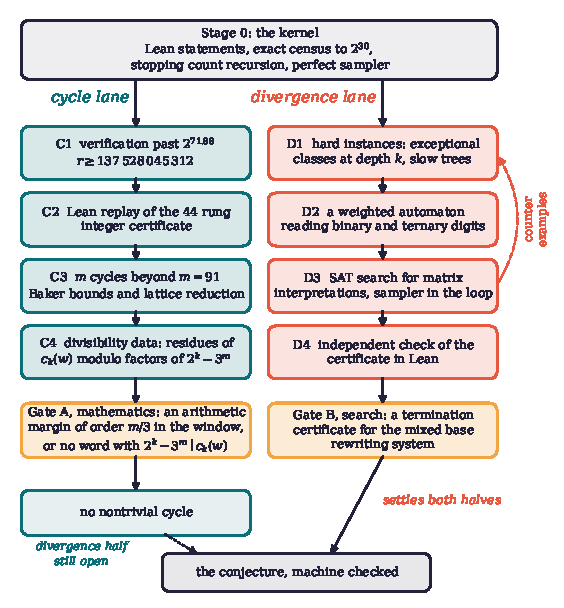
\includegraphics[width=\textwidth]{figures/ch10d_roadmap.pdf}
\caption{A computational road map. The kernel supplies exact tools shared by
both lanes. The cycle lane produces definite partial results at every stage
but needs a mathematical step at Gate A. The divergence lane is a search for a
single certificate; if Gate B is passed, the certificate settles both halves
at once. The dashed loop is the counterexample guided refinement of
\cref{sec:ch10d:lanes}.}
\label{fig:ch10d:roadmap}
\end{figure}

\subsection{Stage 0: the kernel}

The kernel is what the book already provides and what every later stage uses.
It has four parts. The Lean statements of \cref{sec:ch8:lean} fix the trusted
checker and the precise form of the conjecture, of descent and of the absence of nontrivial cycles. The exact census to $2^{30}$
(\cref{sec:ch3:missing}) supplies ground truth for every statistic of
stopping times. The stopping count recursion of \cref{prop:ch2:dp} gives the
exact volume $1-F(k)$ of the exceptional set at every depth in $O(k^2)$
operations. And the perfect sampler of \cref{thm:ch10b:perfect} draws a uniform
exceptional residue at depth $k$ in $O(k)$ operations. The last two together
mean that the hard part of the input space, the classes that have not yet
descended, is a computable and samplable object at every finite depth.

\subsection{The two lanes}\label{sec:ch10d:lanes}

\paragraph{The cycle lane.} Its stages are those of \cref{tab:ch10b:programme},
now ordered by what they buy.

C1 extends verification past $2^{71.884}$. By \cref{tab:ch8:thresholds} the
exact certificate of \cref{thm:cycles} then reaches $r\ge137\,528\,045\,312$ odd elements, the
record that Hercher's sharper accounting already gives at the verified range $2^{71}$; the next threshold is at $2^{75.433}$.
It costs less than twice the effort of the range $2^{71}$ and is pure
engineering. Every extension of the verified range also weakens what \cref{prob:ch11:b1} asks, since the constant $2^{71}$ of \cref{prop:ch9b:bounded} is the verified range.

C2 replays the $44$ rung certificate in Lean, turning
\cref{thm:cycles} into a machine checked theorem (project P1 of \cref{chap:open}).

C3 extends the exclusion of $m$ cycles beyond $m=91$. Each value of $m$ is a
finite computation, a lower bound for a linear form in logarithms followed by
lattice reduction, and each excluded $m$ is a theorem. The cost grows with $m$
and the method has no end point, so C3 produces results but cannot finish.

C4 gathers the data for Gate A. For each admissible shape $(m,k)$ near the rungs
of the ladder, factor $D=2^k-3^m$, and for each prime factor $p$ compute the
set of residues of $c_k(w)$ modulo $p$ over all words with $m$ ones, by the
recursion of \cref{sec:ch10b:cycles} in time proportional to $pkm$. With primes
below $3000$ this excludes only shapes with $m\le8$; the point of C4 is
different. It records, shape by shape, how close the words come to the
divisibility, and so produces the evidence on which a conjecture about the
numbers $c_k(w)$ can be formulated.

Gate A is mathematics. By \cref{cor:ch8:window} an arithmetic improvement of
the upper end of the window by a factor of order $m/3$ excludes all cycles; the
exploration of \cref{chap:cycles} shows that no argument from size alone can
provide it for balanced words. What is needed is a divisibility theorem: no
word $w$ with $m$ ones among $k$ letters has $2^k-3^m\mid c_k(w)$, apart from
the trivial cycle. Computation can find the right statement and test it on all
words up to a moderate length; it cannot supply the proof.

\paragraph{The divergence lane.} This lane is a search for a single
certificate, and if it succeeds it settles the whole conjecture, cycles
included. The reason is the theorem of Yolcu, Aaronson and Heule
(\cref{sec:ch10b:automated}): the Collatz map can be encoded as a string
rewriting system on a mixed binary and ternary representation whose
termination is \emph{equivalent} to the conjecture. A termination proof
excludes divergent orbits and nontrivial cycles alike. Their search found
proofs of nontrivial weakenings but not of the conjecture itself. The book
supplies four pieces of guidance that sharpen the search.

D1 builds the instances that a candidate certificate must survive. The perfect
sampler gives exact uniform draws from the exceptional classes at depth $k$, for
$k$ in the hundreds; the census gives every integer below $2^{30}$ with its
stopping time; and the tree decomposition of \cref{chap:samplers} gives the
slow integers below $2^{26}$ organized into trees of merged orbits, thirty four
of them above level $400$, each represented by the orbit at its root. These are the hardest instances in each sense: the
deepest residues, the slowest integers, and the representatives of
independent slow orbits.

D2 fixes the class of potentials. The ledger dictates three features. The
leading term must be logarithmic, since $x_n$ itself is a martingale and has no
drift (\cref{thm:martingale}). The horizon must vary with $n$, since no fixed
horizon monotone certificate exists (\cref{cor:ch4:multistride}); in a rewriting system
this is automatic, since each rule is local and the number of rewrites is
unbounded. And the potential must read integrality, by
\cref{rem:ch10d:integrality}; in the rewriting encoding this can in principle be supplied by
end markers~\cite{yolcu2023}, which make the leading digit of $n$ visible, and by the ternary
digits, which record the arithmetic of $3n+1$ that binary residues lose. A
matrix interpretation, which assigns to each letter a small matrix and to each
word the product, is a potential that reads the digits of $n$ through a finite
automaton, here one reading both expansions
(\cref{sec:ch10b:automated}). Its dimension $d$ and the size of its entries are
the two parameters of the search.

D3 is the search. For given $d$ and entry bound the existence of a matrix
interpretation under which every rule strictly decreases is a finite
constraint problem, which a SAT or SMT solver decides. The book suggests a
counterexample guided loop around the solver: propose a candidate
interpretation from a cheap relaxation, test it on the hard instances of D1,
add the instances it fails on as constraints, and call the full solver only on
candidates that pass. The loop is the dashed arrow in
\cref{fig:ch10d:roadmap}. Its value is that the hard instances are exact and
cheap to generate in quantity, so the expensive solver is reserved for
candidates that already respect the structure of the problem. The final
certificate does not depend on the instances: a matrix interpretation is
checked rule by rule, and the check is universal.

D4 checks any certificate found, independently of the solver that found it,
in Lean, so that the final theorem rests on the small kernel of Stage 0 and not
on the correctness of a large search program.

Gate B is the existence of a certificate. Nothing guarantees it. Conway's
theorem (\cref{sec:ch1:conway}) shows that no algorithm decides the
termination of every map of Collatz type, so no search procedure can be
promised to succeed on this one; and a certificate, if one exists, may require
a dimension or entry size beyond any feasible search. What the guidance of
D1 and D2 does is to restrict the search to the only class the obstructions
leave open and to make each failed candidate informative.

\subsection{What each stage proves}

\Cref{tab:ch10d:milestones} lists the stages with what each one proves on its
own. The order of work it suggests is as follows. The kernel exists. C1 and C2
are engineering of known cost and should run first and in parallel. D1 is
cheap and already largely built. D2 and D3 are the core of the programme and
the natural place for sustained computation; a pilot on the weakened systems
that Yolcu, Aaronson and Heule did prove terminating is the right benchmark
for the counterexample guided loop, since there the answer is known
(project P10 of \cref{chap:open}). C3 and C4 run alongside, C3 for partial
results and C4 to feed the mathematical step at Gate A.

\begin{table}[!htbp]
\centering\small
\setlength{\tabcolsep}{3pt}
\caption{Stages of the computational path, what each proves on its own, and
its status. Only the gates and B1 would finish a half: Gate B and, given the positive density preprints, B1 would finish both.}
\label{tab:ch10d:milestones}
\begin{tabular}{@{}l>{\raggedright\arraybackslash}p{0.50\textwidth}>{\raggedright\arraybackslash}p{0.32\textwidth}@{}}
\toprule
Stage & What it proves & Status \\
\midrule
0 & exact tools: census, recursion, sampler, Lean statements & in this book \\
C1 & the record $r\ge137\,528\,045\,312$ by the exact certificate & less than twice the work of $2^{71}$ \\
C2 & the bound of \cref{thm:cycles}, machine checked & designed, $44$ rungs \\
C3 & no $m$ cycle for each further $m$ & finite per $m$, no end point \\
C4 & exclusion of shapes; data for a divisibility conjecture & works for $m\le8$ with small primes \\
Gate A & no nontrivial cycle & needs a theorem \\
B1 & the whole conjecture, given the positive density preprints (\cref{prop:ch9b:bounded}) & needs a theorem (\cref{prob:ch11:b1}) \\
D1 & exact hard instances at every depth & built \\
D2 & the admissible class of potentials & specified here \\
D3 & a termination certificate, if one exists in the class & search; pilot first \\
D4 & the conjecture, machine checked & follows D3 \\
Gate B & the whole conjecture & unknown \\
\bottomrule
\end{tabular}
\end{table}

\subsection{What simulation contributes}

The question of \cref{chap:samplers}, whether an energy and a sampler could
find the answer in polynomial time, has a definite place on the path. A
sampler cannot decide the conjecture: the set it would have to reach is the
limit of a nest of measure zero and, if the conjecture is true, contains no
integer. But simulation is polynomial in the depth for exactly the objects the
divergence lane needs. The perfect sampler produces uniform exceptional
residues at depth $k$ at cost $O(k)$, against $1/(1-F(k))$ draws for rejection, of order $e^{Dk}$ up to a power of $k$, with
$D=0.0347$; at depth $400$ that is one draw in place of $8.6\times10^8$. The tree
decomposition says that the slow integers below $2^{26}$ are represented by
a small number of root orbits. Simulation is therefore the instance generator
of the search, and the reason the counterexample guided loop of D3 can be fed
with exact hard cases in quantity.

\section{Summary}\label{sec:ch10d:summary}

The book leaves the conjecture where it found it, open, but with its boundary
drawn more sharply. On the cycle half it gives an exact certificate for the
best bound the classical method can produce, proves that the method can never
finish, and identifies the arithmetic statement that would. On the divergence
half it proves that every argument reading a bounded number of binary digits
must fail, since such an argument cannot see that $n$ is a positive integer, and it records the one transfer
from averages over starting values to single orbits that the book knows, through density one (\cref{cor:ch9b:densityone}), which rests on unrefereed preprints.
The computational path that remains is narrow and definite. It runs through a
search for a termination certificate that reads integrality, in a class of
potentials the obstructions specify, checked independently in a small trusted
kernel. It may not succeed. If it does, the certificate will have the shape the
optimization reading of this book predicts: a logarithmic potential, a
variable horizon, and memory of unbounded arithmetic information.

\section*{Notes}

The equivalence of termination of the mixed base rewriting system with the
conjecture, and the matrix interpretation search, are due to Yolcu, Aaronson and
Heule~\cite{yolcu2023}. The exclusion of $m$ cycles for small $m$ is due to
Simons and de Weger~\cite{simons2005}, extended to $m\le91$ by
Hercher~\cite{hercher2023}, who also holds the record for the cycle length
bound. The counting exponent $0.84$ is due to Krasikov and
Lagarias~\cite{krasikov2003}, and the theorem on almost bounded values to
Tao~\cite{tao2022}. Conway's undecidability theorem is from~\cite{conway1972}.
The integrality principle of \cref{rem:ch10d:integrality} is folklore in the
$2$ adic literature on the problem~\cite{lagarias1985}; the form given here,
as the common source of the obstructions of \cref{tab:ch10d:obstructions},
the ledger itself, and the organization of the computational path with its
counterexample guided search are ours.

\section*{Exercises}

\begin{exercise}
Verify that $-1$, $-5$ and $-17$ lie on cycles of the accelerated map
$T(x)=x/2$ for even $x$ and $T(x)=(3x+1)/2$ for odd $x$, and find the cycles.
Explain why each obstruction of the first family in
\cref{tab:ch10d:obstructions} is consistent with these cycles.
\end{exercise}

\begin{exercise}
Choose three rows of \cref{tab:ch10d:obstructions}. For each, write down the
strongest statement the approach does prove, and check it against the result
cited in the table.
\end{exercise}

\begin{exercise}
Using \cref{tab:ch8:thresholds}, compute how many doublings of the verification
range beyond $2^{68}$ are needed to raise the cycle bound by a factor of $10$,
and explain why the answer is governed by the continued fraction of $\lt$ rather
than by the cost of verification.
\end{exercise}

\begin{exercise}
A matrix interpretation of dimension $1$ assigns to each letter a positive
number and to each word the product of the numbers of its letters. Show that
the weight of a word depends only on how many times each letter occurs, not on
their order. Deduce that such a weight cannot distinguish the binary
expansions of $4j+1$ and $4j+3$ when they have the same digits in a different
order, and use \cref{thm:nolyapunov} to explain why this is a serious defect
for a potential meant to certify descent.
\end{exercise}
